\section{Results}

We implement our \gls{rsp} heuristic algorithm on the aforementioned conceptual aircraft design problem.
Our nominal objective function is total fuel consumption, which is
to be minimized given a payload and a range requirement.

\subsection{Mitigation of probability of failure}

The problem is solved for different sizes of box and elliptical uncertainty sets
by varying the parameter $\Gamma$, as defined in Appendix \ref{LP_to_GP}. Mathematically, for box uncertainty,
$\Gamma$ is a measure of the centered width in logspace of the defined parameter uncertainty, normalized by the
standard deviation of the parameter. For elliptical uncertainty, it is the maximum diameter of the Euclidian norm
ball of $u_i$, which is the number of standard deviations of perturbation of each ith parameter from its nominal value.
Intuitively, it is a measure of how much risk is being hedged against. $\Gamma = 0$
implies that all of the parameters take their nominal values with zero uncertainty,
and larger $\Gamma$ protects against more parameter uncertainty, where a box uncertainty is
more conservative than elliptical uncertainty.

The design variables are then fixed for each solution so that the design can be simulated for
different realizations of the uncertain parameters in Table~\ref{tab:uncertainties}
to examine average design performance. In this~\gls{mc} scheme, the random variables
are simulated from independent and identically distributed $3\sigma$ truncated Gaussians.
We simulate from the truncated Gaussian since this makes it possible to
confirm mathematically that for $\Gamma = 1$, all simulations of uncertain parameters are feasible.
Designs for each solution in Figure~\ref{fig:probOfFailure} are simulated with the same set
of uncertainty realizations for consistency. \\

\begin{figure}[ht]
    \centering
    \captionsetup{justification=centering, font=small}
    \begin{subfigure}{0.49\textwidth}
        \centering
        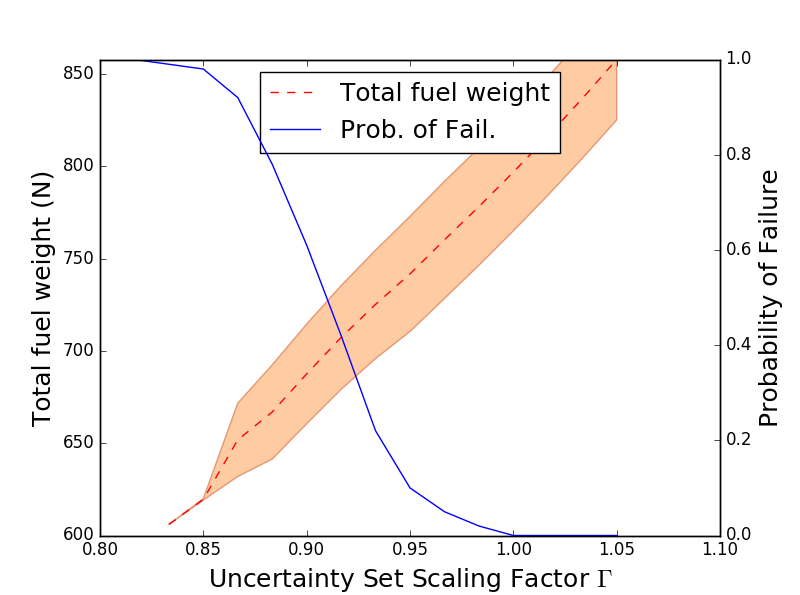
\includegraphics[height=2.3in]{signomial_simple_flight/box_best_pairs.png}
         \caption{Box Uncertainty Set}
    \end{subfigure}%
    ~ 
    \begin{subfigure}{0.49\textwidth}
        \centering
        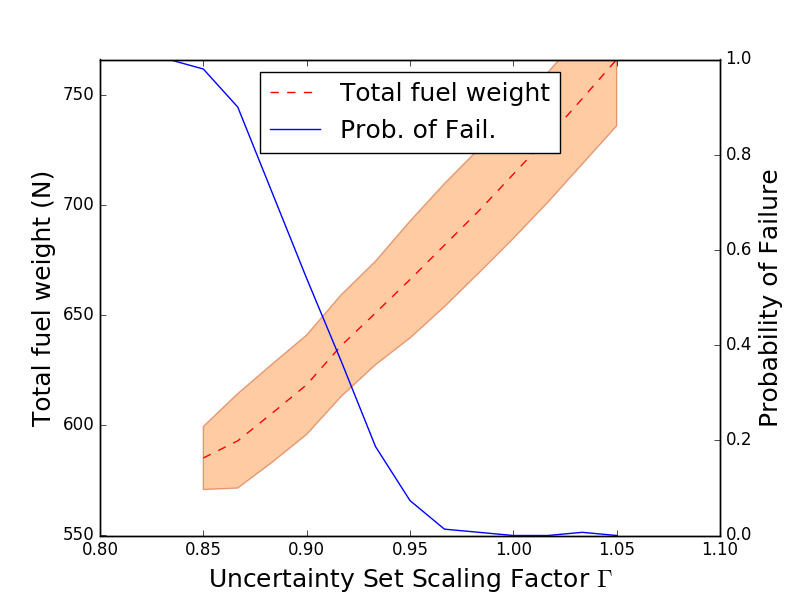
\includegraphics[height=2.3in]{signomial_simple_flight/ell_best_pairs.png}
         \caption{Elliptical Uncertainty Set}
    \end{subfigure}
    \caption{Simulated performance of the optimal robust aircraft, using the Best Pairs formulation,
    as a function of $\Gamma$ for different uncertainty sets.
    The dashed line and the band represent the mean and standard deviation of the performance
    of aircraft designed for different $\Gamma$,
    and simulated with 100 \gls{mc} samples of uncertain parameters. TODO:update.}
    \label{fig:probOfFailure}
\end{figure}

We define the probability of failure of a design as the probability that any constraint
in the design optimization problem is violated in a \gls{mc} simulation.
As expected, Figure \ref{fig:probOfFailure} shows that probability of failure goes to zero as $\Gamma$ increases.
It is noteworthy that, for the nominal problem ($\Gamma = 0$) and for uncertainty up to $\Gamma \leq 0.8$, none of
the 100 simulated uncertain parameters result in feasible solutions. Under uncertain parameters,
the aircraft designed for the average case would almost surely fail to complete its mission.
That being said, it is necessary to sacrifice performance to achieve a high degree ($3\sigma$) of
reliability as in the solution for $\Gamma = 1$.

\begin{table}[!h]
\begin{center}
\caption{\label{tab:results} SP Aircraft Optimization Results TODO:update}
\begin{tabular}{c c c c c}
\hline
Free variable & Units & No Uncert. & Box [$\Gamma = 1.0$] & Elliptical [$\Gamma = 1.0$] \\
\hline
$L/D$ & - & 40.3 & 31.2 & 34.0 \\
$AR$ & - & 22.6 & 11.8 & 14.5 \\
$Re$ & - & $1.80 \times 10^6$ & $3.59 \times 10^7$ & $3.00 \times 10^6$ \\
$S$ & $\mathrm{m^2}$ & 18.1 & 40.2 & 37.4 \\
$V$ & $\mathrm{m/s}$ & 41.5 & 40.3 & 38.8 \\
$T_{flight}$ & $\mathrm{hr}$ & 20.6 & 21.3 & 22.1 \\
$W_w$ & $\mathrm{N}$ & 2960 & 5060 & 4830 \\
$W_{w,strc}$ & $\mathrm{N}$ & 1880 & 2410 & 2360 \\
$W_{w,surf}$ & $\mathrm{N}$ & 1080 & 2650 & 2470 \\
$V_{f,avail}$ & $\mathrm{m^3}$ & 0.063 & 0.111 & 0.100 \\
$V_{f,fuse}$ & $\mathrm{m^3}$ & 0.005 & 0 & 0 \\
$V_{f,wing}$ & $\mathrm{m^3}$ & 0.058 & 0.111 & 0.100 \\
\hline
E[Objective] & Units & No Uncert. & Box [$\Gamma = 1.0$] & Elliptical [$\Gamma = 1.0$] \\
\hline
$W_{fuel}$ & $\mathrm{N}$ & 502 & 893 & 803 \\
\hline
P[failure] & & No Uncert. & Box [$\Gamma = 1.0$] & Elliptical [$\Gamma = 1.0$] \\
\hline
\% & & 100 & 0 & 0\\
\hline
\end{tabular}
\end{center}
\end{table}

% TODO: update diagrams and graphs with solutions for the problem with composite objective

Moreover, using margins would in the best case be as good as using a box uncertainty set, and therefore will lead
to a more conservative solution with inferior performance.

Figure~\ref{compare_signomial} compares the different methodologies in terms of setup and
run times. Since the setup time of the nominal problem is minimal, we have
normalized the results by the run time of the nominal problem for comparison.
The bottom axis ranks the methods by their level of conservativeness (Best Pairs
and Simple Conservative formulations being the least and most conservative respectively),
and the elliptical formulations are less conservative than the box formulations~\cite{Saab2018}.
For the box uncertainty, solution times increase for increasing levels of conservativeness,
whereas for the elliptical uncertainty they decrease.
%The Best Pairs and Linearized Perturbations methods achieve good performance,
%however the Best Pairs methodology needs the most number of constraints,
%while the Linearized perturbations requires the most setup and solve time.
%The Simple Conservative formulation is significantly faster than the other formulations
%and requires the least number of additional constraints.

\ \\
\begin{figure}[ht]
    \centering
    \captionsetup{justification=centering, font=small}
    \begin{subfigure}{0.49\textwidth}
        \centering
        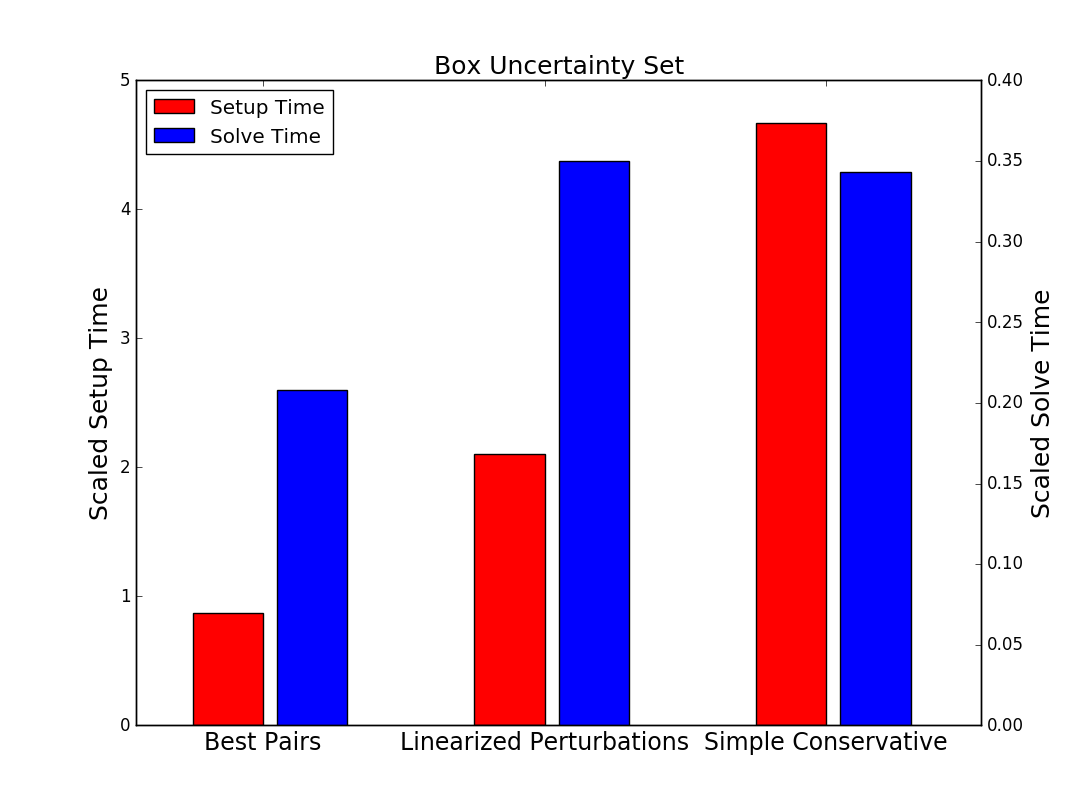
\includegraphics[height=2.3in]{signomial_simple_flight/box_times.png}
    \end{subfigure}
    ~
    \begin{subfigure}{0.49\textwidth}
        \centering
        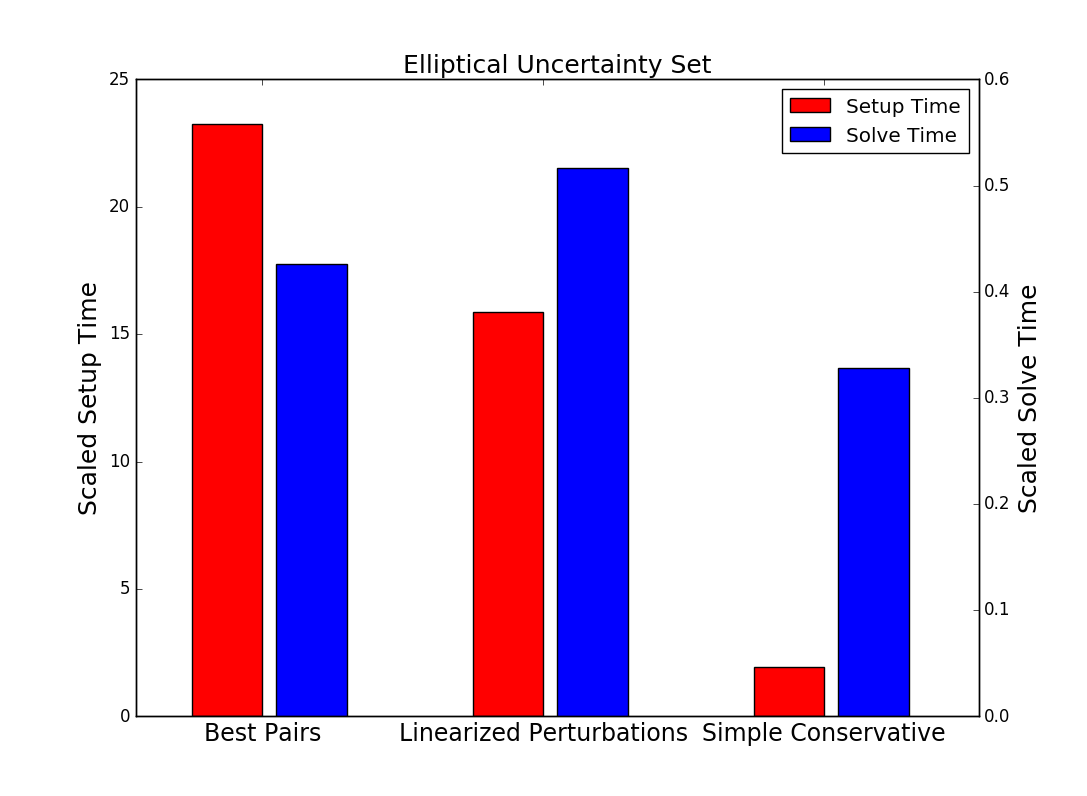
\includegraphics[height=2.3in]{signomial_simple_flight/ell_times.png}
    \end{subfigure}
    \caption{Robust signomial simple aircraft solution and setup times, normalized by the
    nominal problem solution time, for $\Gamma = 1$.
    Note that the problems with box uncertainty have much lower setup
    time costs versus those with elliptical uncertainty. TODO:update.}
    \label{compare_signomial}
\end{figure}

\subsection{The Effect of Robustness on Multiobjective Performance}

One of the benefits of convex and difference-of-convex optimization methods is the ability to optimize for
different objectives~\cite{York2018}. As a demonstration, we optimized the aircraft without uncertainty
for 7 different objectives, and show
the non-dimensionalized results in Table~\ref{tab:nondimresults}.

\begin{table}
    \resizebox{\textwidth}{!}{
    \csvautobooktabularcenter{figures/objective_table.csv}
    }
\caption{Non-dimensionalized variations in objective values with respect to the aircraft optimized
for different objectives. Objective values were normalized by the total fuel solution.}
    \label{tab:nondimresults}
\end{table}

Since the model is physics based, it is able to accommodate a range of objectives,
even ones that are not often considered such as aspect ratio. The resulting aircraft
also differ drastically with respect to performance and design variables.
As the most extreme example,
the aircraft optimized for time cost has 150 times the engine weight as the aircraft
optimized for total fuel, since a huge amount of power is required to fly fast.

Aside from this caricature example, we further demonstrate the capabilities of \gls{rsp}s in
multiobjective design by considering a more realistic scenario.
We perform the optimization of the aircraft with no uncertainty and ellipsoidal uncertainty ($\Gamma = 1$)
for 4 different objective functions, and plot the results on spider plots.
Spider plots are useful because they allow engineers to see the performance of
different designs in a multi-objective
environment. One way to envision the multi-objective
performance of the aircraft is to consider the area contained within the web defined by the aircraft's
performance; the smaller the web area the better.
Due to the large disparities in the potential values of design variables depending
on objective as shown in Table~\ref{tab:nondimresults}, we chose to demonstrate this using four objective functions
that would be expected to have a high degree of correlation and therefore yield similar aircraft designs. These were
 total (time and fuel) cost, total fuel, takeoff weight and mid-cruise lift-over-drag (L/D).

\begin{figure}
    \begin{center}
    \begin{tikzpicture}
        \node[inner sep=0] (center) at (0,0)
        {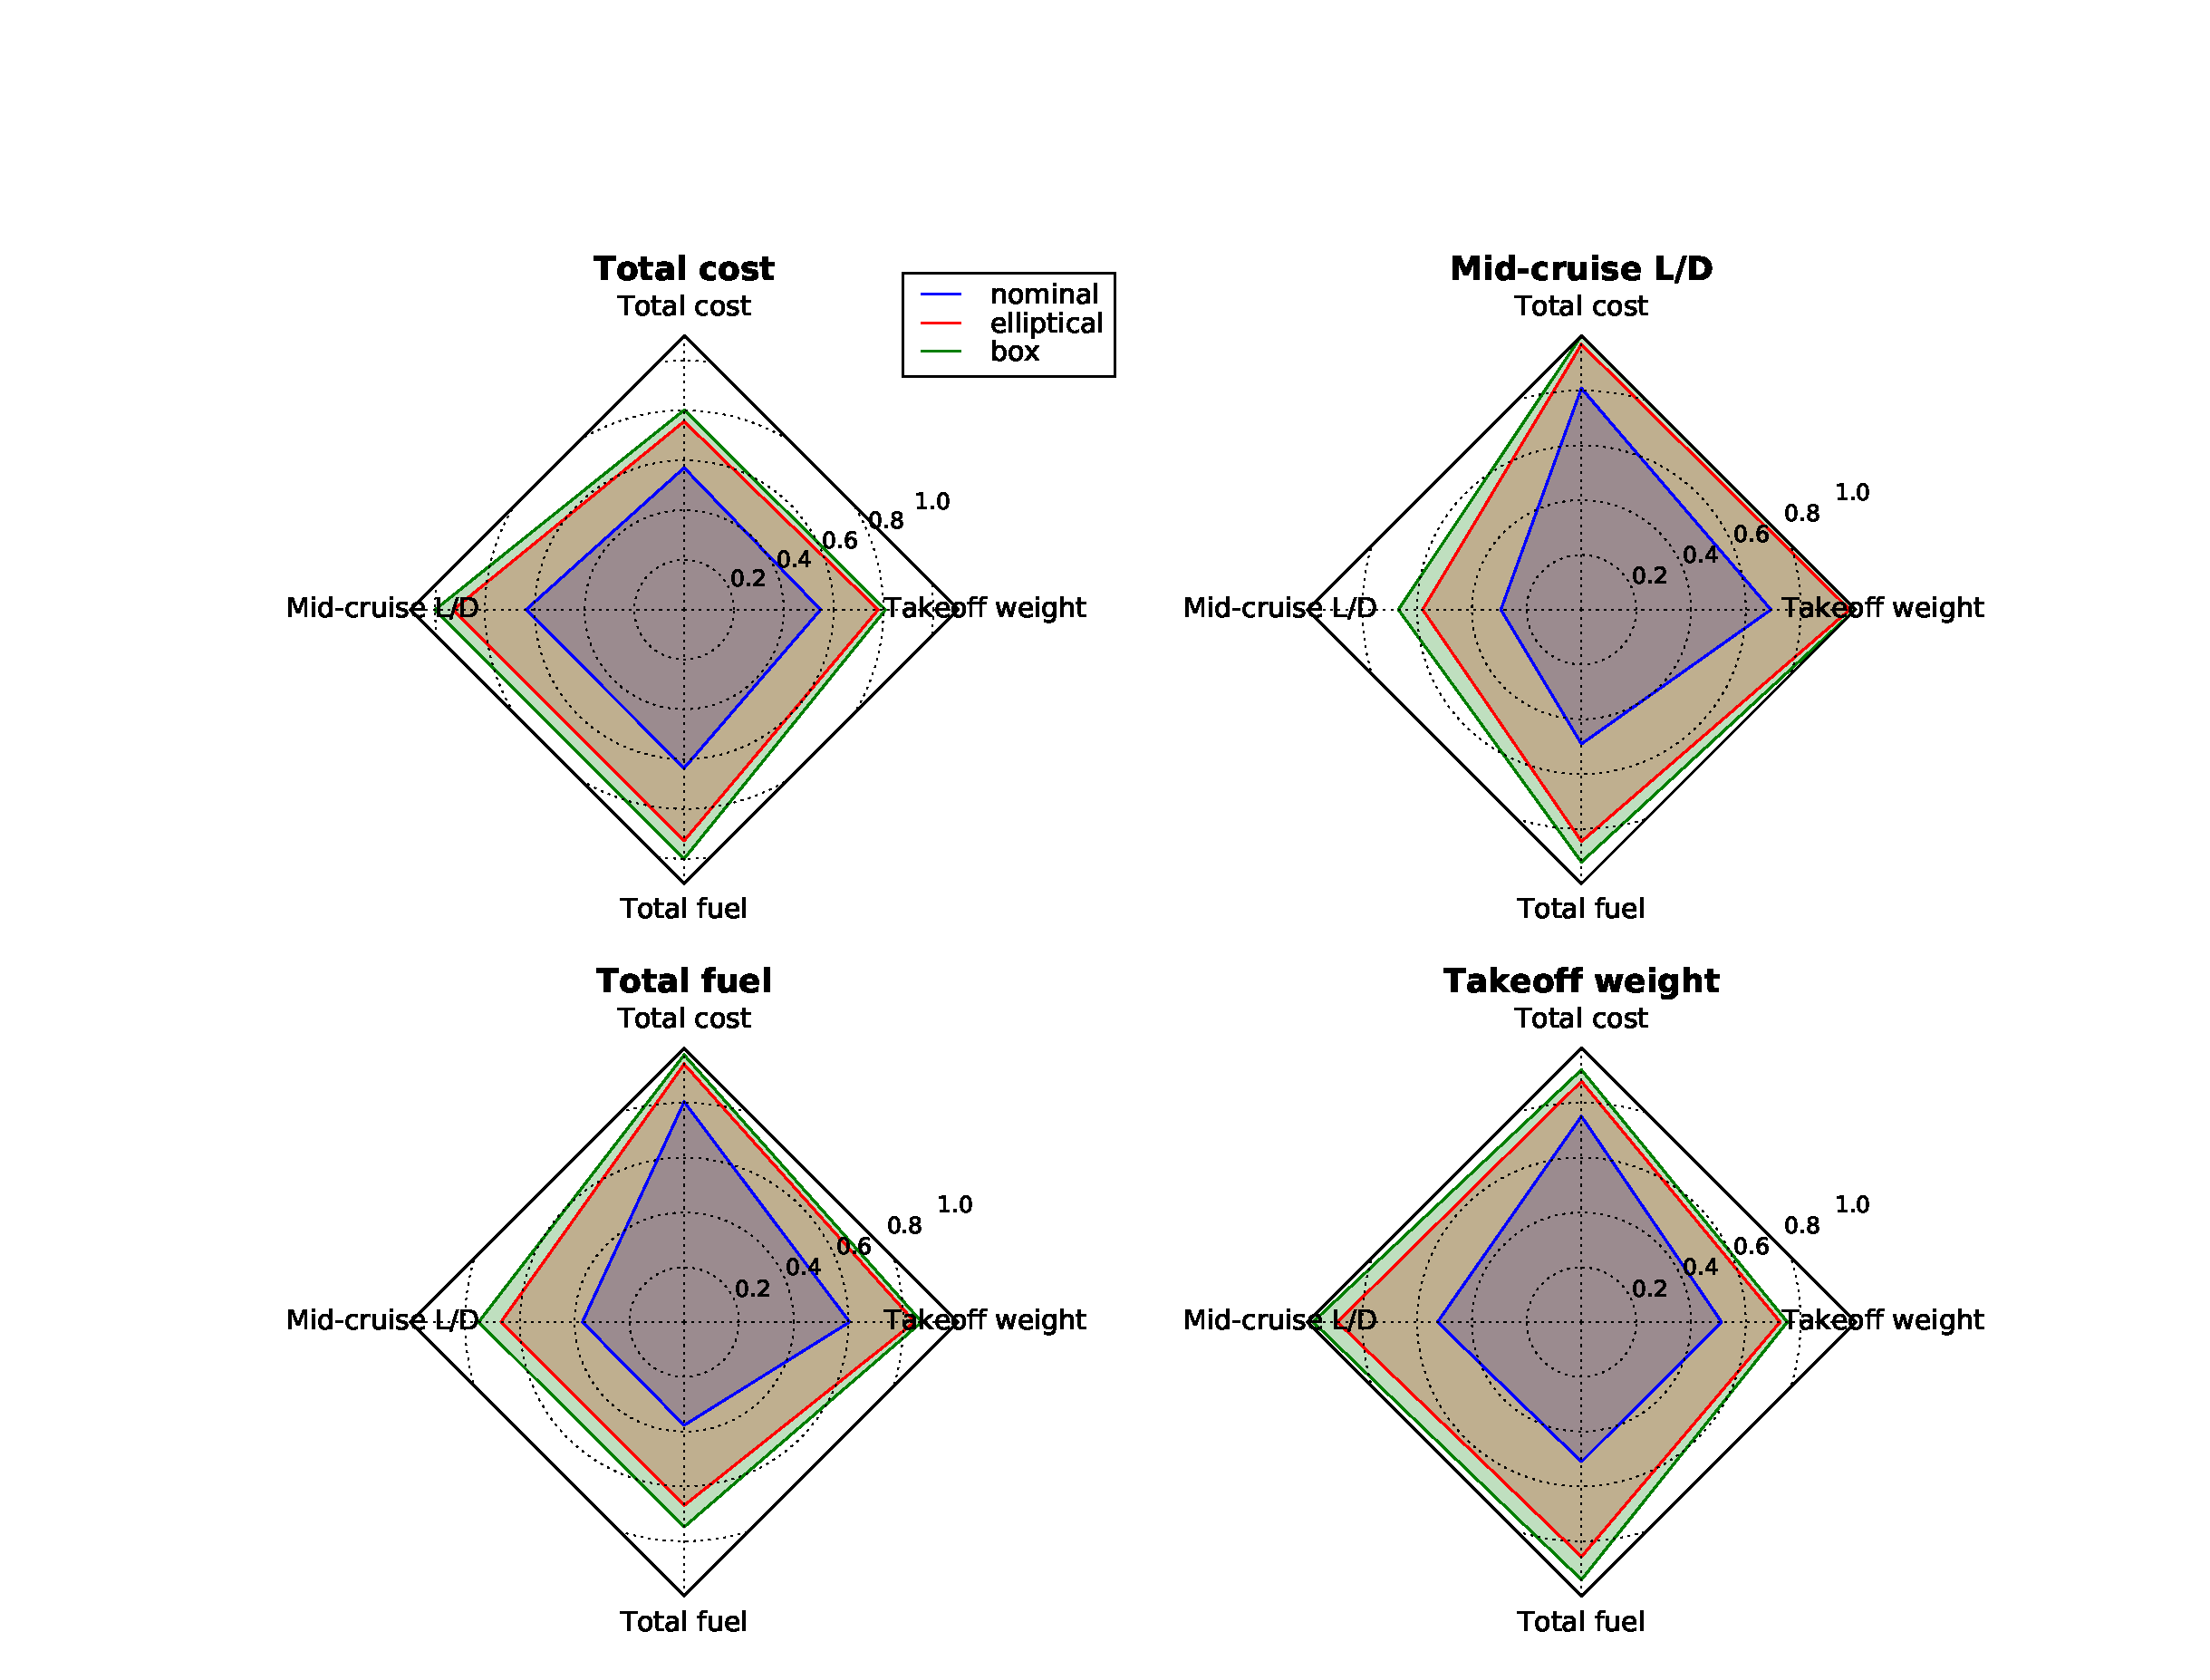
\includegraphics[trim={2cm 0 1cm 0},clip]{figures/4objradar.pdf}};
        \node[inner sep=0] (ul) at (-1.0, 0.25)
        {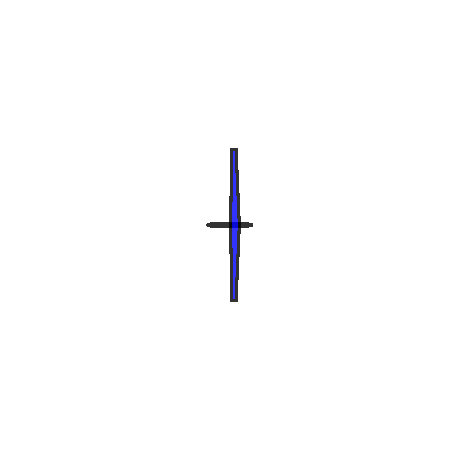
\includegraphics[height=3.8cm]{figures/2nominal.pdf}};
        \node[inner sep=0] (ur) at (1.0, 0.25)
        {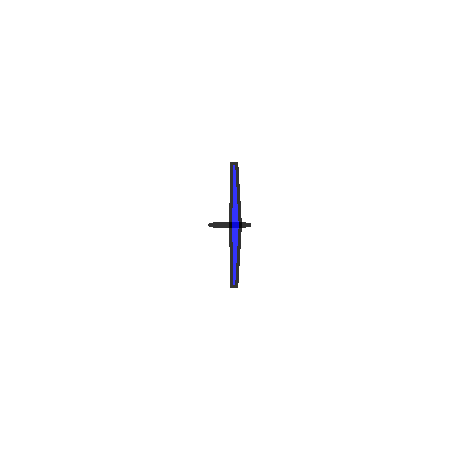
\includegraphics[height=3.8cm]{figures/3nominal.pdf}};
        \node[inner sep=0] (ll) at (-1.0, -2)
        {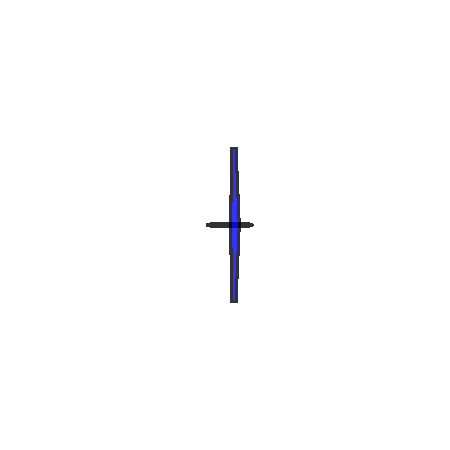
\includegraphics[height=3.8cm]{figures/0nominal.pdf}};
        \node[inner sep=0] (lr) at (1.0, -2)
        {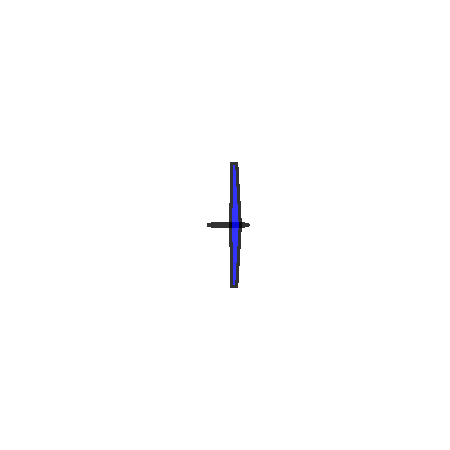
\includegraphics[height=3.8cm]{figures/1nominal.pdf}};
    \end{tikzpicture}
    \caption{The spider plots of aircraft performance, for aircraft optimized for different objectives.
    The bolded titles are the design objectives for each plot, whereas the individual spiderwebs
    show the non-dimensionalized multiobjective performance of the aircraft designed under different
    uncertainty sets.}
    \label{fig:spider}
\end{center}
\end{figure}

\begin{figure}
    \begin{center}
        \begin{subfigure}{0.4\linewidth}
            \begin{tikzpicture}
                \node[inner sep=0] (l) at (-2.5,0)
                {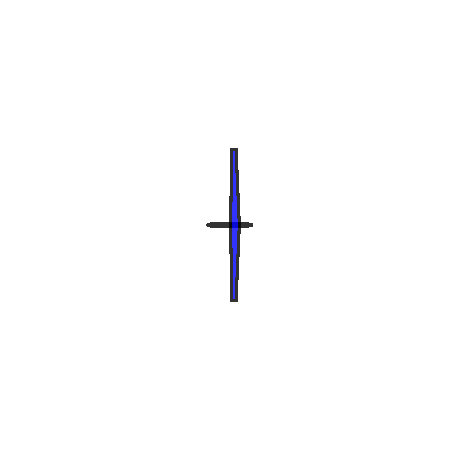
\includegraphics[height=5cm]{figures/2nominal.pdf}};
                \node[inner sep=0] (c) at (-1,0)
                {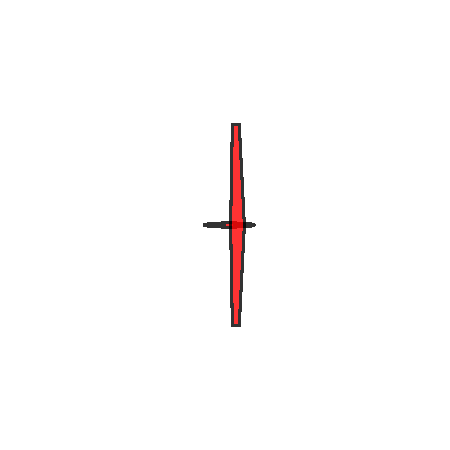
\includegraphics[height=5cm]{figures/2elliptical.pdf}};
                \node[inner sep=0] (r) at (.5,0)
                {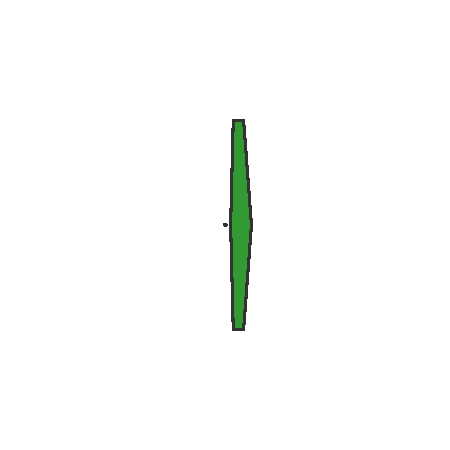
\includegraphics[height=5cm]{figures/2box.pdf}};
            \end{tikzpicture}
            \caption{Total cost}
        \end{subfigure}
        \begin{subfigure}{0.4\linewidth}
            \begin{tikzpicture}
                \node[inner sep=0] (l) at (-2.5,0)
                {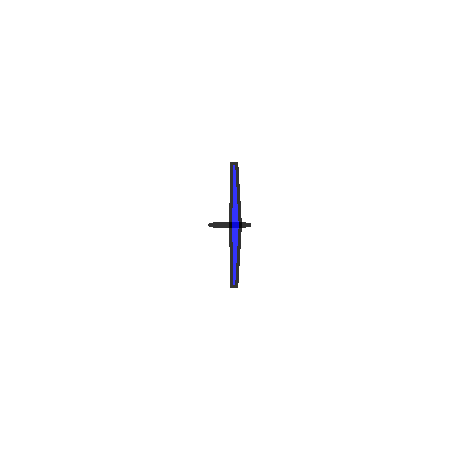
\includegraphics[height=5cm]{figures/3nominal.pdf}};
                \node[inner sep=0] (c) at (-1,0)
                {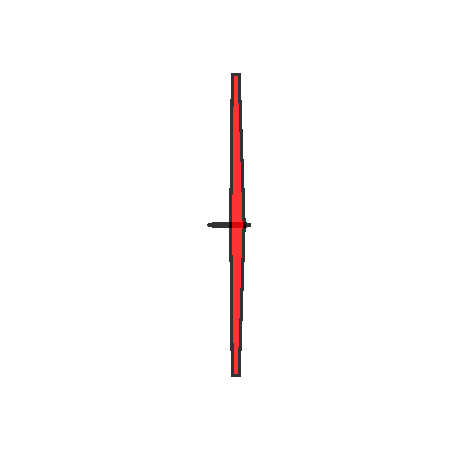
\includegraphics[height=5cm]{figures/3elliptical.pdf}};
                \node[inner sep=0] (r) at (.5,0)
                {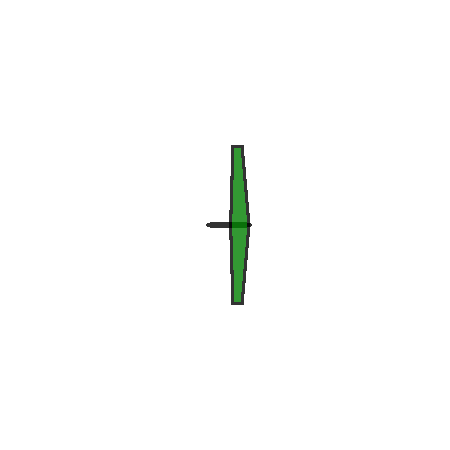
\includegraphics[height=5cm]{figures/3box.pdf}};
            \end{tikzpicture}
            \caption{Mid-cruise L/D}
        \end{subfigure}
        \begin{subfigure}{0.4\linewidth}
            \begin{tikzpicture}
                \node[inner sep=0] (l) at (-2.5,0)
                {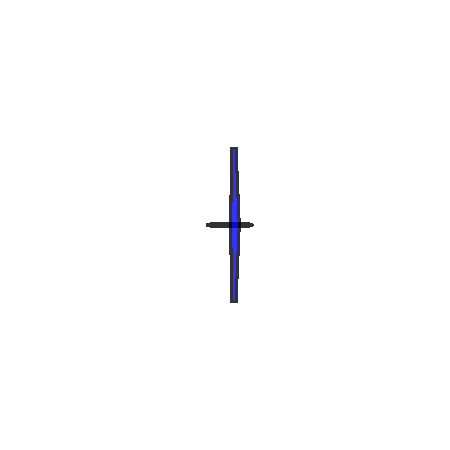
\includegraphics[height=5cm]{figures/0nominal.pdf}};
                \node[inner sep=0] (c) at (-1,0)
                {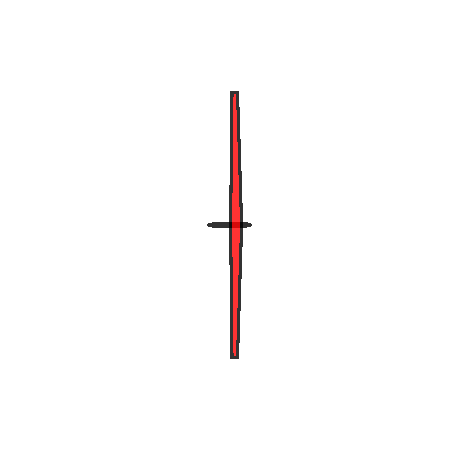
\includegraphics[height=5cm]{figures/0elliptical.pdf}};
                \node[inner sep=0] (r) at (.5,0)
                {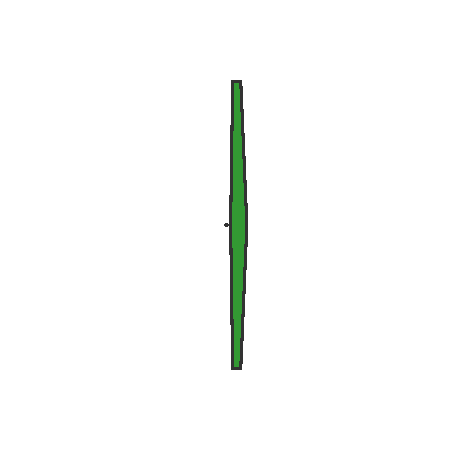
\includegraphics[height=5cm]{figures/0box.pdf}};
            \end{tikzpicture}
            \caption{Total fuel}
        \end{subfigure}
        \begin{subfigure}{0.4\linewidth}
            \begin{tikzpicture}
                \node[inner sep=0] (l) at (-2.5,0)
                {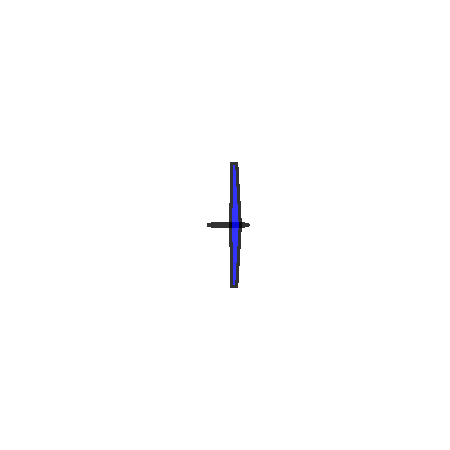
\includegraphics[height=5cm]{figures/1nominal.pdf}};
                \node[inner sep=0] (c) at (-1,0)
                {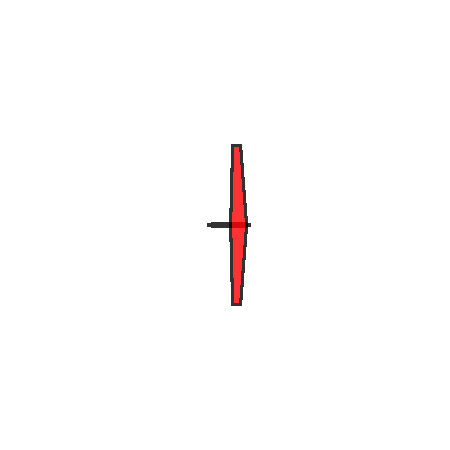
\includegraphics[height=5cm]{figures/1elliptical.pdf}};
                \node[inner sep=0] (r) at (.5,0)
                {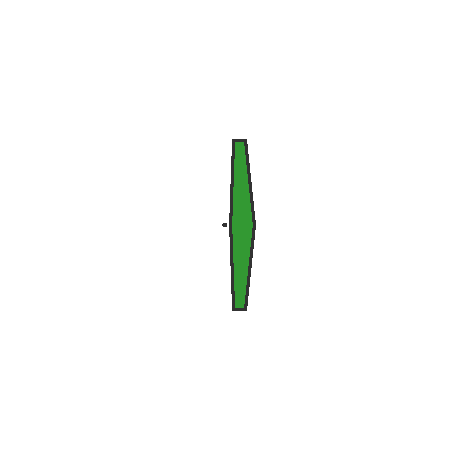
\includegraphics[height=5cm]{figures/1box.pdf}};
            \end{tikzpicture}
            \caption{Takeoff weight}
        \end{subfigure}
        \caption{Sketches of the aircraft drawn for corresponding spider plots. Drawn to scale for comparison.}
    \end{center}
\end{figure}

In the spider plots in Figure~\ref{fig:spider}, it is possible to see the effect of robustness on
the different worst-case performance metrics of the different aircraft. In this example, four objectives that
are highly coupled were chosen to make sure the we can do a comparative graphical analysis.
For the nominal case, it is possible to see that
the aircraft designed for total fuel performs the best when all four objectives are considered,
assuming that all objectives are weighted equally. As expected,
the box uncertainty set is strictly more conservative than the elliptical uncertainty set, for
all objectives. In this case, it is true that total fuel is the objective that maximizes
the multiobjective outcome, but for certain \gls{rsp}s it is possible that the multiobjective behavior
of aircraft designed using different uncertainty sets

And interestingly enough, there is a convergence in the geometry of the aircraft as they are designed
to be robust to uncertain outcomes. All of the robust designs eschew the storage of fuel in the fuselage
for larger wings that can store more fuel. This is not to say that none of the aircraft will ever have
fuselages; one example is a mission where flight time is a much more important objective
than fuel weight.

% TODO: add robust cases where there is a fuselage.


In absence of understanding of the role of uncertainty in aircraft design,

TODO: flesh out.
This analysis could also be performed for the mean performance
of the aircraft determined through ~\gls{mc} simulation, but this demonstration limits
its scope to the worst-case analysis.

\subsection{Risk minimization problems}

All of the previous multi-objective analyses have assumed that we have an
understanding of exactly how much risk we are
willing to tolerate. However, it would also make sense if risk was the objective of our
model. This would suggest the following formulation:

\begin{align*}
    \text{max} &~\Gamma \\
    \text{s.t.}     &~f_i(x,u) \leq 0, i = 1,\ldots,n \\
                    & \norm{u} \leq \Gamma \\
                    &~f_0(x) \leq (1+\delta)f_0^*,~\delta \geq 0 \tag{a}
    \label{eq:goalprogramming}
\end{align*}

where $f_0^*$ is the optimum of the nominal problem in Formulation~\ref{eq:normform}, $\delta$
is a fractional measure of the objective that we are willing to sacrifice for robustness, which
gives $(1+\delta)f_0^*$ as the upper bound on the objective value. Intuitively,
this is a form of goal programming,
where we specify the exact maximum worst-case value of an objective we can tolerate so that the program
risk is acceptable, but in the meanwhile maximize the total size of the uncertainty we can handle.
We call the method of minimizing an objective for set ${\Gamma}$ \emph{the $\Gamma$ method},
while we call the goal programming approach, which maximizes $\Gamma$ for a set $\delta$,
\emph{the $\delta$ method}.

The problem in Formulation~\ref{eq:goalprogramming} is not equivalent to the problem in Formulation~\ref{eq:normform},
but should yield the same result. As a proof of concept, we perform the same probability of failure
analysis as in Figure~\ref{fig:deltaVsGamma}, but have the objective bound be an input to the
optimization problem and the $\Gamma$ of the uncertainty set be maximized.

\begin{figure}[ht]
    \centering
    \captionsetup{justification=centering, font=small}
    \begin{subfigure}{0.49\textwidth}
        \centering
        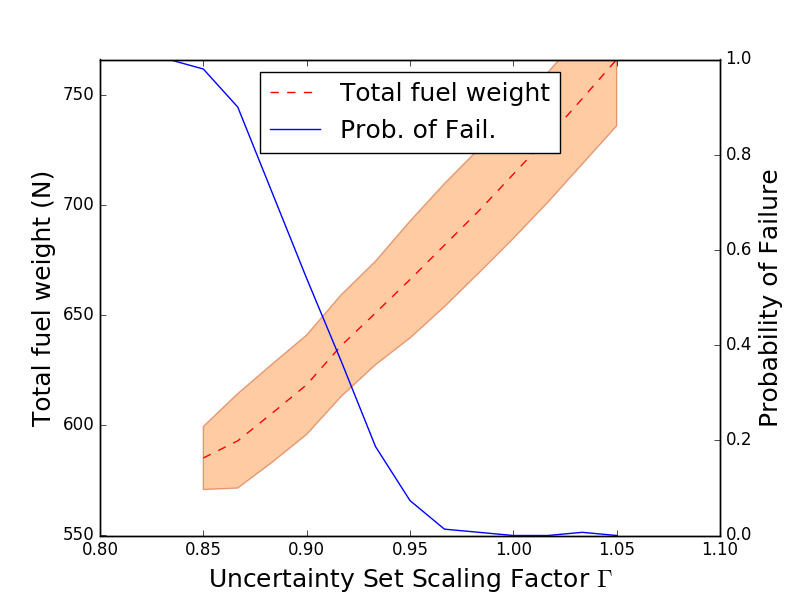
\includegraphics[height=2.3in]{signomial_simple_flight/ell_best_pairs.png}
         \caption{Elliptical Uncertainty, $\Gamma$ method}
    \end{subfigure}%
    ~
    \begin{subfigure}{0.49\textwidth}
        \centering
        \includegraphics[height=2.3in]{signomial_simple_flight/deltaResults.png}
         \caption{Elliptical Uncertainty, $\delta$ method}
    \end{subfigure}
    \caption{Simulated performance of the optimal robust aircraft, using the Best Pairs formulation
    for the $\Gamma$ and $\delta$ methods.
    The dashed line and the band represent the mean and standard deviation of the performance
    of aircraft designed for different $\Gamma$,
    and simulated with 100 \gls{mc} samples of uncertain parameters. TODO:update.}
    \label{fig:deltaVsGamma}
\end{figure}

As expected, we get identical results from the outputs of the two formulations (to confirm).
We can also expand this framework to perform multivariate goal programming,
by changing (a) in the formulation~\ref{eq:goalprogramming} to include all
objectives we are interested in.

\begin{align*}
    f_{0,j}(x) \leq (1+\delta_j) f^*_{0,j},~\delta_j \geq 0,~j = 1,\ldots, m
    \label{eq:multigoal}
\end{align*}

The benefit of goal programming is that it allows us to explore multidisciplinary tradeoffs without
having to enumerate the design space along each objective direction.
In design it is not obvious whether an objective should in fact be a constraint instead. The most
fundamental choice that an engineer can make in design is what the objective function is, and it is
often the case that there are many potential objectives that are conflicting. The term multiobjective optimization is misleading
because you can only optimize for one objective at once,
and the design is going to be influenced by how engineers weight different objectives.
Risk minimization makes these implicit decisions explicit, empowers engineers to choose
how much performance they would be willing to sacrifice with respect
to optimal but fragile designs to obtain robust designs, and gives a prediction of the margin of error
for every parameter that they have to make designs feasible.

\section{Potential Future Work or Studies}

There are a myriad of potential extensions to signomial programming under uncertainty.
In the spirit of helping reduce program risk in aerospace design,
the authors make a few observations and recommendations.

In this study, we do not discriminate between the kinds of constraints violated. However, it would
be possible to rank the severity of constraint violations so as to penalize some (eg. structural safety)
more heavily than others (maximum range constraint). This would inject further realism into the
design under uncertainty since some violations contribute to program risk more
strongly than others.

Another potentially valuable extension to the proposed framework is the concurrent implementation
of multiple sets to contain the uncertain parameters, with the purpose of restricting uncertain
outcomes further. One example of this would be to impose an  L1-norm on the integer number of uncertain parameters
as well as an L2-norm on the overall size of uncertainty set
This method can be used to set the total size of the uncertainty set in a Euclidian sense,
but then also to restrict the stochasticity to a subset of all of the uncertain parameters,
thereby somewhat restricting nature. This also turns the problem into an integer robust
optimization problem which poses interesting computational challenges.

With respect to interesting studies, \gls{ro} opens up many possibilities to discover and analyze the benefits
of adaptable architectures in aircraft design versus more traditional point designs
when faced with parametric uncertainty. Some examples of these are modular designs, morphing designs,
adaptively manufactured designs and aircraft families. It is likely that these types of engineered
robustness become more effective at reducing program risk in presence of uncertainty, since they are more likely
to deliver value under adverse stochastic outcomes.

In situations where there is data available to aid design, \gls{ro} can help explore
the design space while taking into account the stochasticity and noise in the data.
This opens up an array of potential trade studies where engineers can learn about
the exposure of designs to the sparsity and spread of data and attempt to gather
data which best reduces the uncertainty in the performance of optimal designs.
